\documentclass{article}
\usepackage{graphicx}
\usepackage{hyperref}
\usepackage{listings}
\usepackage{enumitem}

\title{Final Assignment \\ Computer Workshop Course}
\author{Your Name}
\date{\today}

\begin{document}
\maketitle
\tableofcontents
\newpage

\section{Exploration Task}

\subsection{Vim Advanced Features}
Explore and document 3 advanced features of Vim that were not covered in class.

\subsubsection{Macros}
\begin{itemize}
    \item \textbf{Description:} Macros allow you to record a sequence of commands and replay them.
    \item \textbf{How to Use:}
    \begin{enumerate}
        \item Start recording a macro by pressing \texttt{q} followed by a register name (e.g., \texttt{a}).
        \item Perform the sequence of commands you want to record.
        \item Stop recording by pressing \texttt{q} again.
        \item Replay the macro by pressing \texttt{@} followed by the register name (e.g., \texttt{@a}).
    \end{enumerate}
    \item \textbf{Example:} Record a macro to delete a line and paste it below:
    \begin{lstlisting}[language=bash]
    qa dd p q
    \end{lstlisting}
    Replay it with \texttt{@a}.
\end{itemize}

\subsubsection{Marks}
\begin{itemize}
    \item \textbf{Description:} Marks allow you to save positions in a file and quickly jump back to them.
    \item \textbf{How to Use:}
    \begin{enumerate}
        \item Set a mark by pressing \texttt{m} followed by a letter (e.g., \texttt{ma} to set mark \texttt{a}).
        \item Jump to a mark by pressing \texttt{'} followed by the letter (e.g., \texttt{'a}).
    \end{enumerate}
    \item \textbf{Example:} Set a mark at the top of a file (\texttt{ma}), scroll down, and return to the mark (\texttt{'a}).
\end{itemize}

\subsubsection{Global Commands}
\begin{itemize}
    \item \textbf{Description:} The \texttt{:g} command allows you to perform actions on lines matching a pattern.
    \item \textbf{How to Use:}
    \begin{itemize}
        \item Syntax: \texttt{:g/pattern/command}
        \item Example: Delete all lines containing the word "TODO":
        \begin{lstlisting}[language=bash]
        :g/TODO/d
        \end{lstlisting}
    \end{itemize}
\end{itemize}

\subsection{Memory Profiling}
This semester, you got to know about dynamic memory allocation in C in your Programming Fundamentals class.

\subsubsection{Memory Leak}
\begin{itemize}
    \item \textbf{What is a Memory Leak?}
    A memory leak occurs when a program allocates memory (e.g., using \texttt{malloc} in C) but fails to release it (e.g., using \texttt{free}). Over time, this can cause the program to consume more and more memory, leading to performance degradation or crashes.
    \item \textbf{How It Happens:}
    \begin{itemize}
        \item Forgetting to call \texttt{free} after \texttt{malloc}.
        \item Losing the pointer to the allocated memory (e.g., reassigning the pointer without freeing the original memory).
    \end{itemize}
\end{itemize}

\subsubsection{Memory Profilers (Valgrind)}
\begin{itemize}
    \item \textbf{What is Valgrind?}
    Valgrind is a tool for detecting memory leaks, memory errors, and profiling programs. It is widely used for debugging C and C++ programs.
    \item \textbf{How It Helps:}
    \begin{itemize}
        \item Detects memory leaks by tracking all memory allocations and deallocations.
        \item Identifies invalid memory accesses (e.g., reading/writing freed memory).
        \item Provides detailed reports to help pinpoint issues.
    \end{itemize}
    \item \textbf{Example Usage:}
    \begin{lstlisting}[language=bash]
    valgrind --leak-check=full ./your_program
    \end{lstlisting}
\end{itemize}

\subsection{GNU/Linux Bash Scripting}
In this section, you will get to know some handy bash utilities.

\subsubsection{fzf}
\begin{itemize}
    \item \textbf{What is Fuzzy Searching?}
    Fuzzy searching is a technique for finding items that approximately match a search pattern, even if the pattern contains typos or is incomplete. It is useful for quickly locating files, commands, or other data.
    \item \textbf{Install fzf:}
    \begin{lstlisting}[language=bash]
    sudo apt install fzf  # On Debian/Ubuntu
    brew install fzf     # On macOS
    \end{lstlisting}
    \item \textbf{What Does \texttt{ls | fzf} Do?}
    \begin{itemize}
        \item Lists all files in the current directory using \texttt{ls}.
        \item Pipes the output to \texttt{fzf}, which allows you to interactively search and select a file.
    \end{itemize}
\end{itemize}

\subsubsection{Using fzf to Find Your Favorite PDF}
\begin{itemize}
    \item \textbf{List All PDF Files:}
    Use the \texttt{fd} command to list all PDF files recursively:
    \begin{lstlisting}[language=bash]
    fd -e pdf
    \end{lstlisting}
    \item \textbf{Select a PDF Using fzf:}
    Pipe the output of \texttt{fd} to \texttt{fzf} for interactive selection:
    \begin{lstlisting}[language=bash]
    fd -e pdf | fzf
    \end{lstlisting}
\end{itemize}

\subsubsection{Opening the File Using Zathura}
\begin{itemize}
    \item \textbf{Command to Open the Selected PDF:}
    Use \texttt{zathura} with command substitution to open the selected PDF:
    \begin{lstlisting}[language=bash]
    zathura $(fd -e pdf | fzf)
    \end{lstlisting}
    \item \textbf{Explanation:}
    \begin{itemize}
        \item \texttt{\$(...)} runs the command inside and substitutes its output.
        \item \texttt{fd -e pdf | fzf} selects a PDF file.
        \item \texttt{zathura} opens the selected file.
    \end{itemize}
\end{itemize}

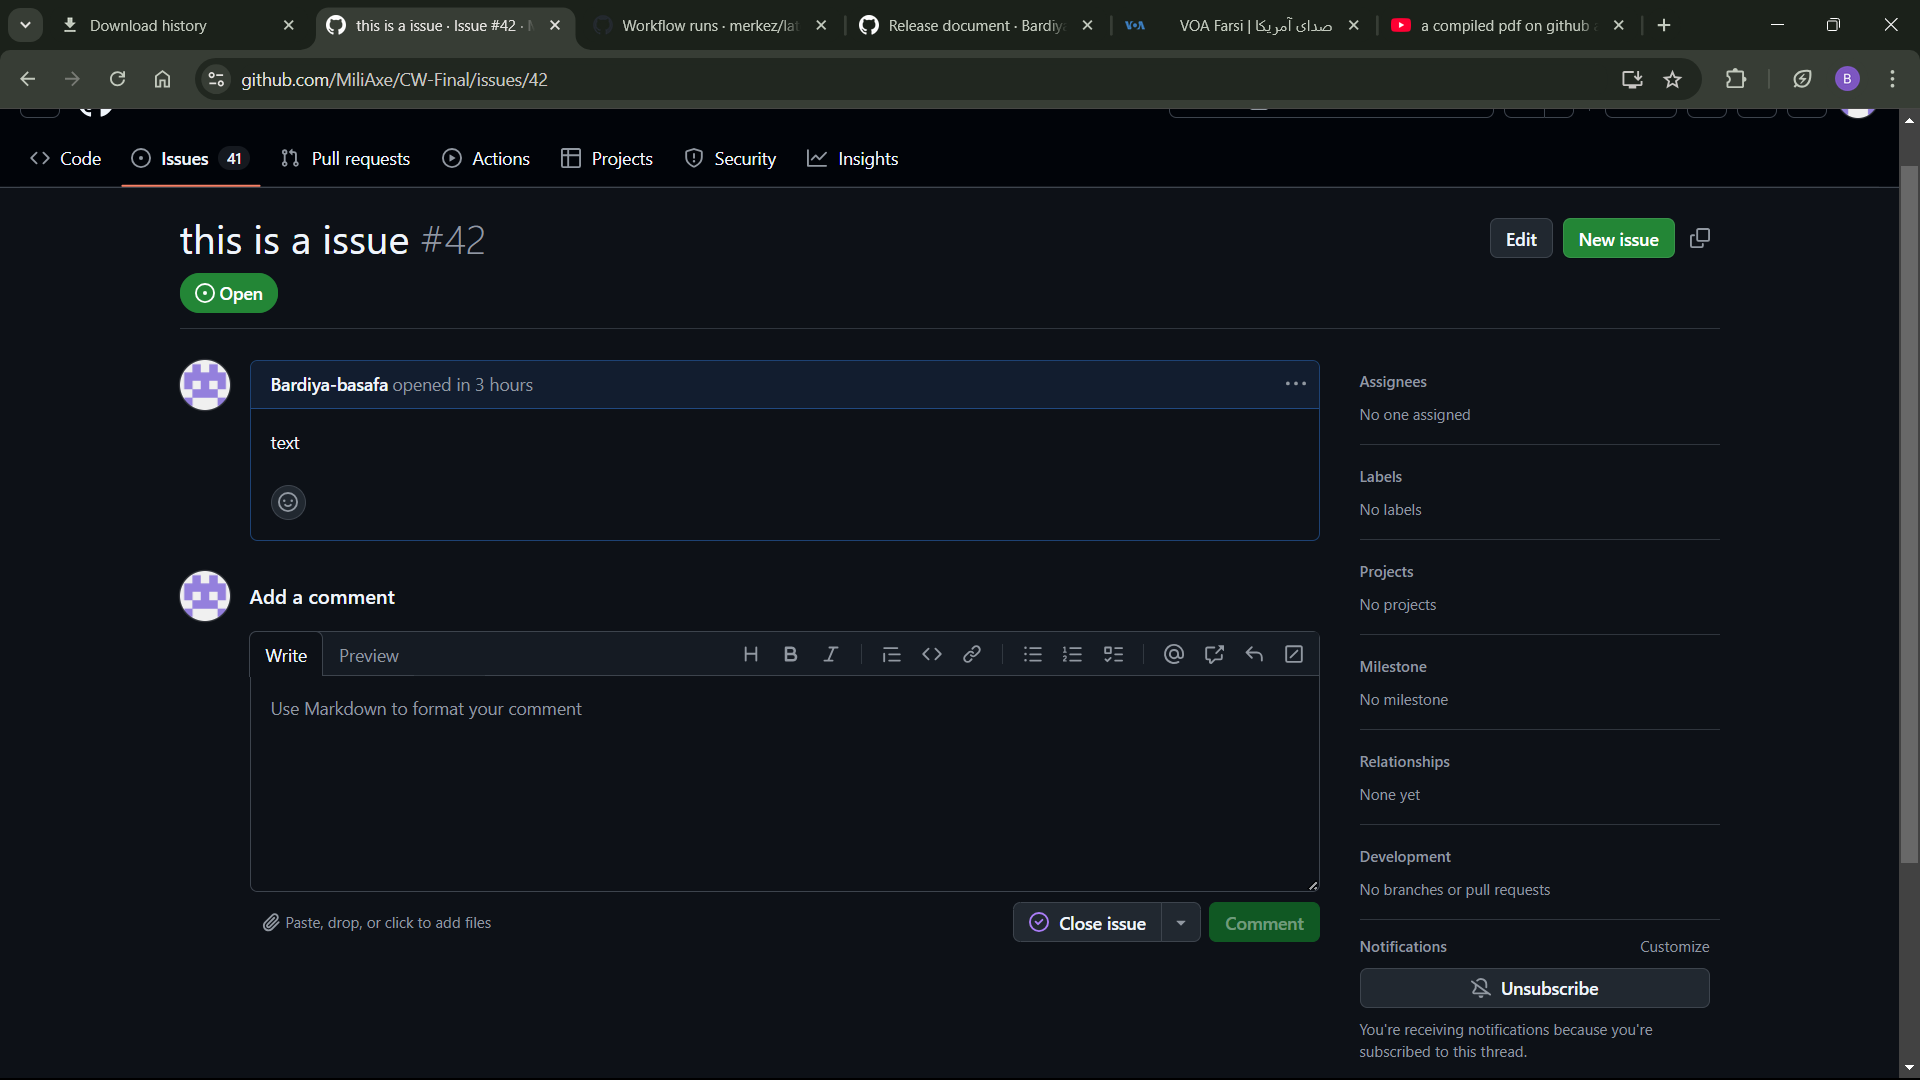
\includegraphics{image.png}

\end{document}
